\documentclass[twoside]{book}

% Packages required by doxygen
\usepackage{fixltx2e}
\usepackage{calc}
\usepackage{doxygen}
\usepackage{graphicx}
\usepackage[utf8]{inputenc}
\usepackage{makeidx}
\usepackage{multicol}
\usepackage{multirow}
\PassOptionsToPackage{warn}{textcomp}
\usepackage{textcomp}
\usepackage[nointegrals]{wasysym}
\usepackage[table]{xcolor}

% NLS support packages
\usepackage[italian]{babel}

% Font selection
\usepackage[T1]{fontenc}
\usepackage{mathptmx}
\usepackage[scaled=.90]{helvet}
\usepackage{courier}
\usepackage{amssymb}
\usepackage{sectsty}
\renewcommand{\familydefault}{\sfdefault}
\allsectionsfont{%
  \fontseries{bc}\selectfont%
  \color{darkgray}%
}
\renewcommand{\DoxyLabelFont}{%
  \fontseries{bc}\selectfont%
  \color{darkgray}%
}
\newcommand{\+}{\discretionary{\mbox{\scriptsize$\hookleftarrow$}}{}{}}

% Page & text layout
\usepackage{geometry}
\geometry{%
  a4paper,%
  top=2.5cm,%
  bottom=2.5cm,%
  left=2.5cm,%
  right=2.5cm%
}
\tolerance=750
\hfuzz=15pt
\hbadness=750
\setlength{\emergencystretch}{15pt}
\setlength{\parindent}{0cm}
\setlength{\parskip}{0.2cm}
\makeatletter
\renewcommand{\paragraph}{%
  \@startsection{paragraph}{4}{0ex}{-1.0ex}{1.0ex}{%
    \normalfont\normalsize\bfseries\SS@parafont%
  }%
}
\renewcommand{\subparagraph}{%
  \@startsection{subparagraph}{5}{0ex}{-1.0ex}{1.0ex}{%
    \normalfont\normalsize\bfseries\SS@subparafont%
  }%
}
\makeatother

% Headers & footers
\usepackage{fancyhdr}
\pagestyle{fancyplain}
\fancyhead[LE]{\fancyplain{}{\bfseries\thepage}}
\fancyhead[CE]{\fancyplain{}{}}
\fancyhead[RE]{\fancyplain{}{\bfseries\leftmark}}
\fancyhead[LO]{\fancyplain{}{\bfseries\rightmark}}
\fancyhead[CO]{\fancyplain{}{}}
\fancyhead[RO]{\fancyplain{}{\bfseries\thepage}}
\fancyfoot[LE]{\fancyplain{}{}}
\fancyfoot[CE]{\fancyplain{}{}}
\fancyfoot[RE]{\fancyplain{}{\bfseries\scriptsize Generato Ven 30 Giu 2017 19\+:09\+:28 per Linear-\/\+Regression da Doxygen }}
\fancyfoot[LO]{\fancyplain{}{\bfseries\scriptsize Generato Ven 30 Giu 2017 19\+:09\+:28 per Linear-\/\+Regression da Doxygen }}
\fancyfoot[CO]{\fancyplain{}{}}
\fancyfoot[RO]{\fancyplain{}{}}
\renewcommand{\footrulewidth}{0.4pt}
\renewcommand{\chaptermark}[1]{%
  \markboth{#1}{}%
}
\renewcommand{\sectionmark}[1]{%
  \markright{\thesection\ #1}%
}

% Indices & bibliography
\usepackage{natbib}
\usepackage[titles]{tocloft}
\setcounter{tocdepth}{3}
\setcounter{secnumdepth}{5}
\makeindex

% Hyperlinks (required, but should be loaded last)
\usepackage{ifpdf}
\ifpdf
  \usepackage[pdftex,pagebackref=true]{hyperref}
\else
  \usepackage[ps2pdf,pagebackref=true]{hyperref}
\fi
\hypersetup{%
  colorlinks=true,%
  linkcolor=blue,%
  citecolor=blue,%
  unicode%
}

% Custom commands
\newcommand{\clearemptydoublepage}{%
  \newpage{\pagestyle{empty}\cleardoublepage}%
}


%===== C O N T E N T S =====

\begin{document}

% Titlepage & ToC
\hypersetup{pageanchor=false,
             bookmarks=true,
             bookmarksnumbered=true,
             pdfencoding=unicode
            }
\pagenumbering{roman}
\begin{titlepage}
\vspace*{7cm}
\begin{center}%
{\Large Linear-\/\+Regression \\[1ex]\large v 0.\+1 }\\
\vspace*{1cm}
{\large Generato da Doxygen 1.8.8}\\
\vspace*{0.5cm}
{\small Ven 30 Giu 2017 19:09:28}\\
\end{center}
\end{titlepage}
\clearemptydoublepage
\tableofcontents
\clearemptydoublepage
\pagenumbering{arabic}
\hypersetup{pageanchor=true}

%--- Begin generated contents ---
\chapter{Indice dei moduli}
\section{Moduli}
Questo è l'elenco di tutti i moduli\+:\begin{DoxyCompactList}
\item \contentsline{section}{Basic\+Fixed\+Point\+Operation}{\pageref{group___basic_fixed_point_operation}}{}
\begin{DoxyCompactList}
\item \contentsline{section}{Truncation}{\pageref{group___truncation}}{}
\end{DoxyCompactList}
\end{DoxyCompactList}

\chapter{Design Unit Index}
\section{Design Unit List}
Here is a list of all design unit members with links to the Entities they belong to\+:\begin{DoxyCompactList}
\item\contentsline{section}{entity \hyperlink{classadder}{adder} }{\pageref{classadder}}{}
\item\contentsline{section}{architecture \hyperlink{classtb__adder_1_1behavior}{behavior} }{\pageref{classtb__adder_1_1behavior}}{}
\item\contentsline{section}{architecture \hyperlink{classtb__generic__cla__adder_1_1behavior}{behavior} }{\pageref{classtb__generic__cla__adder_1_1behavior}}{}
\item\contentsline{section}{architecture \hyperlink{classtb___linear_regression_1_1_behavioral}{Behavioral} }{\pageref{classtb___linear_regression_1_1_behavioral}}{}
\item\contentsline{section}{entity \hyperlink{classcla__adder__cell}{cla\+\_\+adder\+\_\+cell} \\*Cella base di un addizionatore con carry-\/lookahead.

La cella somma tra loro due addendi ed un carry in ingresso, tutti espressi su un solo bit. Oltre a generare la somma, genera le funzioni \char`\"{}propagazione\char`\"{} e \char`\"{}generazione\char`\"{} del carry }{\pageref{classcla__adder__cell}}{}
\item\contentsline{section}{entity \hyperlink{classcla__carry__net}{cla\+\_\+carry\+\_\+net} \\*Rete logica di calcolo dei riporti per un addizionatore a quattro bit con carry lookahead.

Permette di anticipare il calcolo dei riporti usando le funzioni \char`\"{}propagazione\char`\"{} e \char`\"{}generazione\char`\"{} prodotte dai singoli blocchi \hyperlink{classcla__adder__cell}{cla\+\_\+adder\+\_\+cell}, in modo da ridurre tempo necessario ad effettuare il calcolo di tutti i carry, quindi il tempo necessario a completare la somma. Questo blocco calcola solo i carry, pertanto va connesso ai blocchi \hyperlink{classcla__adder__cell}{cla\+\_\+adder\+\_\+cell}, per il calcolo materiale della somma, così come indicato dallo schema seguente, il quale rappresenta lo schema completo di un addizionatore a quattro bit\+:  }{\pageref{classcla__carry__net}}{}
\item\contentsline{section}{architecture \hyperlink{classcla__adder__cell_1_1dataflow}{dataflow} }{\pageref{classcla__adder__cell_1_1dataflow}}{}
\item\contentsline{section}{architecture \hyperlink{classcla__carry__net_1_1dataflow}{dataflow} \\*Implementazione dataflow dell\textquotesingle{}entita\textquotesingle{} \hyperlink{classcla__carry__net}{cla\+\_\+carry\+\_\+net}.

L\textquotesingle{}implementazione si basa sul seguente ragionamento\+: Proviamo ad esprimere, adesso, il carry carryout(i+1) in base alle funzioni gen(i) e prop(i), partendo, ad esempio, da carryout(1). Il carry carryout(0) varra\textquotesingle{} 1 se al passo precedente è stato generato riporto oppure se verra\textquotesingle{} propagato il carry carryin. In formule\+: \begin{center}carryout(0)=genin+(propin$\ast$carryin);\end{center}  Possiamo estendere lo stesso ragionamento a carryout(2)\+: \begin{center}carryout(1)=gen(1)+prop(1)$\ast$carryout(1)=gen(1)+prop(1)$\ast$gen(0)+prop(1)$\ast$prop(0)$\ast$carryin\end{center}  Cio\textquotesingle{} significa che il riporto carryout(1) lo si può esprimere sulla base di soli dati di ingresso con reti combinatorie a due livelli, senza utilizzare valori calcolati da nodi precedenti. Tutto ciò si traduce in un minor tempo necessario ad effettuare il calcolo di tutti i carry, quindi un minor tempo necessario a completare la somma. Purtroppo non si può procedere in questo modo ad oltranza per cui si tende a spezzare" la rete per il calcolo dei carry in blocchi più piccoli, ad esempio reti per il calcolo di carry per quattro bit. Considerando che \begin{center}carryout(4)=gen(3)+prop(3)$\ast$carryout(3)=...=genout+propout$\ast$carryin\end{center}  con \begin{center}genout=gen(3)+(prop(3)$\ast$gen(2))+(prop(3)$\ast$prop(2)$\ast$gen(1))+(prop(3)$\ast$prop(2)$\ast$prop(1)$\ast$gen(0))+(prop(3)$\ast$prop(2)$\ast$prop(1)$\ast$prop(0)$\ast$genin)\end{center}  \begin{center}propout=prop(3)$\ast$prop(2)$\ast$prop(1)$\ast$prop(0)$\ast$propin\end{center}  Si può costruire dei blocchi che presentino in uscita i segnali genout e propout, in modo da permettere ad eventuali blocchi successivi il calcolo veloce dei carry sulla base di questi segnali e del segnale carryin }{\pageref{classcla__carry__net_1_1dataflow}}{}
\item\contentsline{section}{entity \hyperlink{classgeneric__cla__adder}{generic\+\_\+cla\+\_\+adder} \\*Adder custom con carry-\/lookahead

\hyperlink{classgeneric__cla__adder}{generic\+\_\+cla\+\_\+adder} somma tra loro due addendi ed un carry in ingresso; gli addendi sono espressi su multipli interi di quattro bit. Oltre a generare la somma, genera il flag di carry ed il flag di overflow }{\pageref{classgeneric__cla__adder}}{}
\item\contentsline{section}{entity \hyperlink{class_linear_regression}{Linear\+Regression} }{\pageref{class_linear_regression}}{}
\item\contentsline{section}{entity \hyperlink{classmultiplier}{multiplier} }{\pageref{classmultiplier}}{}
\item\contentsline{section}{entity \hyperlink{classnibble__adder}{nibble\+\_\+adder} \\*Addizionatore con carry-\/lookahead a quattro bit.

La cella somma tra loro due addendi ed un carry in ingresso; gli addendi sono espressi su quattro bit. Oltre a generare la somma, genera le funzioni \char`\"{}propagazione\char`\"{} e \char`\"{}generazione\char`\"{} del carry per eventuali blocchi \hyperlink{classnibble__adder}{nibble\+\_\+adder} posti a valle }{\pageref{classnibble__adder}}{}
\item\contentsline{section}{architecture \hyperlink{classmultiplier_1_1_structural}{Structural} \\*Per il prodotto viene utilizzato l\textquotesingle{}operatore $\ast$. La sintesi viene lasciata al particolare sintetizzatore }{\pageref{classmultiplier_1_1_structural}}{}
\item\contentsline{section}{architecture \hyperlink{classadder_1_1structural}{structural} \\*Implementazione mista structural per l\textquotesingle{}entity adder.

A seconda del valore del parametro use\+\_\+custom, verrà istanziato
\begin{DoxyItemize}
\item un sommatore full-\/custom \hyperlink{classgeneric__cla__adder}{generic\+\_\+cla\+\_\+adder}, se use\+\_\+custom = true;
\item un sommatore la cui implementazione è stabilita dal sintetizzatore, se use\+\_\+custom = false; Nel caso in cui venga istanziato il sommatore custom, è richiesto che il numero di bit con il quale sono espressi gli addendi, e di conseguenza quello in vui verrà espressa la loro somma, sia multiplo di quattro 
\end{DoxyItemize}}{\pageref{classadder_1_1structural}}{}
\item\contentsline{section}{architecture \hyperlink{classnibble__adder_1_1structural}{structural} \\*Implementazione structural dell\textquotesingle{}entità \hyperlink{classnibble__adder}{nibble\+\_\+adder}.

Questa architettura istanzia una entità \hyperlink{classcla__carry__net}{cla\+\_\+carry\+\_\+net} ed una entità \hyperlink{classcla__adder__cell}{cla\+\_\+adder\+\_\+cell} per ogni bit su cui sono espressi gli addendi, connettendoli tra loro secondo lo schema riportato di seguito\+:  }{\pageref{classnibble__adder_1_1structural}}{}
\item\contentsline{section}{architecture \hyperlink{class_linear_regression_1_1_structural}{Structural} \\*8 

M\+U\+L\+T1, M\+U\+L\+T2, M\+U\+L\+T3, M\+U\+L\+T4, A\+D\+D5, A\+D\+D6, M\+U\+L\+T6 

Verificare che il troncamento post M\+U\+L\+T6 venga effettuato correttamente (7 bit in testa e 17 in coda) 

C=b\char`\"{}011000011101000101011010\char`\"{}~\newline
 Sum2=b\char`\"{}001010111100110111101111\char`\"{}~\newline
 B=b\char`\"{}001000110100010101100111\char`\"{}~\newline
 Sum1=b\char`\"{}001101001011110110010011\char`\"{}~\newline
 A=b\char`\"{}000111101111000111001010\char`\"{}  

mult2\+\_\+out=b\char`\"{}000001100000100100000111110011100100011000101001\char`\"{}~\newline
 P2= b\char`\"{}000010010000011111001110\char`\"{}~\newline
 mult4\+\_\+out=b\char`\"{}000101000010011011110110000000101010100010101110\char`\"{}~\newline
 P4= b\char`\"{}001010000100110111101100\char`\"{}~\newline
 add2\+\_\+out= b\char`\"{}001100010101010110111010\char`\"{}~\newline
 S6= b\char`\"{}000110001010101011011101\char`\"{}~\newline
 mult1\+\_\+out=b\char`\"{}00001101101100000101101010110\char`\"{}~\newline
 P3= b\char`\"{}011011011000001011010101\char`\"{}~\newline
 mult3\+\_\+out=b\char`\"{}000001110100010000110111011010011110010100100101\char`\"{}~\newline
 P1= b\char`\"{}110100010000110111011010\char`\"{}~\newline
 S5= b\char`\"{}001111101001000010101111\char`\"{}~\newline
 mult6\+\_\+out=b\char`\"{}000000101111101101010010001101101101111101100010\char`\"{}~\newline
 q =b\char`\"{}011111011010100100011011\char`\"{}  

mult2\+\_\+out=b\char`\"{}000001100000100100000111110011100100011000101001\char`\"{}~\newline
 P2= b\char`\"{}000010010000011111001110\char`\"{}~\newline
 mult4\+\_\+out=b\char`\"{}000101000010011011110110000000101010100010101110\char`\"{}~\newline
 P4= b\char`\"{}001010000100110111101100\char`\"{}~\newline
 add2\+\_\+out= b\char`\"{}001100010101010110111010\char`\"{}~\newline
 S6= b\char`\"{}000110001010101011011101\char`\"{}~\newline
 mult1\+\_\+out=b\char`\"{}00001101101100000101101010110\char`\"{}~\newline
 P3= b\char`\"{}011011011000001011010101\char`\"{}~\newline
 mult3\+\_\+out=b\char`\"{}000001110100010000110111011010011110010100100101\char`\"{}~\newline
 P1= b\char`\"{}110100010000110111011010\char`\"{}~\newline
 S5= b\char`\"{}001111101001000010101111\char`\"{}~\newline
 mult6\+\_\+out=b\char`\"{}000000101111101101010010001101101101111101100010\char`\"{}~\newline
 q =b\char`\"{}       011111011010100100011011\char`\"{}  

Superato  }{\pageref{class_linear_regression_1_1_structural}}{}
\item\contentsline{section}{architecture \hyperlink{classgeneric__cla__adder_1_1structural}{structural} \\*Implementazione structural di \hyperlink{classgeneric__cla__adder}{generic\+\_\+cla\+\_\+adder}.

Questa implementazione istanzia tanti blocchi \hyperlink{classnibble__adder}{nibble\+\_\+adder} quanti siano i nibble in cui sono rappresentati gli addendi. La somma è espressa sullo stesso numero di bit. I diversi blocchi sono connessi tra loro come indicato nello schema ricordato di seguito\+:  }{\pageref{classgeneric__cla__adder_1_1structural}}{}
\item\contentsline{section}{entity \hyperlink{classtb__adder}{tb\+\_\+adder} }{\pageref{classtb__adder}}{}
\item\contentsline{section}{entity \hyperlink{classtb__generic__cla__adder}{tb\+\_\+generic\+\_\+cla\+\_\+adder} }{\pageref{classtb__generic__cla__adder}}{}
\item\contentsline{section}{entity \hyperlink{classtb___linear_regression}{tb\+\_\+\+Linear\+Regression} }{\pageref{classtb___linear_regression}}{}
\end{DoxyCompactList}

\chapter{Indice dei file}
\section{File List}
Here is a list of all files with brief descriptions\+:\begin{DoxyCompactList}
\item\contentsline{section}{Src/\hyperlink{truncate_8vhd}{truncate.\+vhd} }{\pageref{truncate_8vhd}}{}
\end{DoxyCompactList}

\chapter{Documentazione dei moduli}
\hypertarget{group___basic_fixed_point_operation}{\section{Basic\+Fixed\+Point\+Operation}
\label{group___basic_fixed_point_operation}\index{Basic\+Fixed\+Point\+Operation@{Basic\+Fixed\+Point\+Operation}}
}


Operazioni fixed-\/point basilari.  


Diagramma di collaborazione per Basic\+Fixed\+Point\+Operation\+:\nopagebreak
\begin{figure}[H]
\begin{center}
\leavevmode
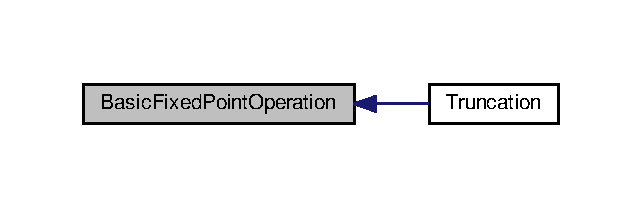
\includegraphics[width=308pt]{group___basic_fixed_point_operation}
\end{center}
\end{figure}
\subsection*{Moduli}
\begin{DoxyCompactItemize}
\item 
\hyperlink{group___truncation}{Truncation}
\begin{DoxyCompactList}\small\item\em Operazione di troncamento. \end{DoxyCompactList}\end{DoxyCompactItemize}


\subsection{Descrizione dettagliata}
Operazioni fixed-\/point basilari. 


\hypertarget{group___truncation}{\section{Truncation}
\label{group___truncation}\index{Truncation@{Truncation}}
}


Operazione di troncamento.  


Diagramma di collaborazione per Truncation\+:\nopagebreak
\begin{figure}[H]
\begin{center}
\leavevmode
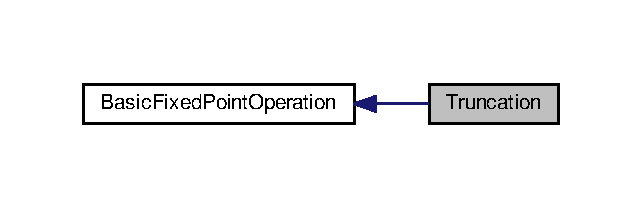
\includegraphics[width=308pt]{group___truncation}
\end{center}
\end{figure}
\subsection*{Entities}
\begin{DoxyCompactItemize}
\item 
\hyperlink{classtruncate}{truncate} entity
\begin{DoxyCompactList}\small\item\em Tronca un segnale di ingresso, espresso in uno specifico formato. \end{DoxyCompactList}\item 
\hyperlink{classtruncate_1_1dataflow}{dataflow} architecture
\end{DoxyCompactItemize}
\subsection*{Constants}
 \begin{DoxyCompactItemize}
\item 
\hypertarget{group___truncation_ga63701d8af27da7452a7588efcff357bc}{\hyperlink{group___truncation_ga63701d8af27da7452a7588efcff357bc}{x} {\bfseries \textcolor{vhdlchar}{integer}\textcolor{vhdlchar}{ }\textcolor{vhdlchar}{ }\textcolor{vhdlchar}{\+:}\textcolor{vhdlchar}{=}\textcolor{vhdlchar}{ }\textcolor{vhdlchar}{ }\textcolor{vhdlchar}{ }\textcolor{vhdlchar}{ }{\bfseries \hyperlink{group___truncation_gabe72b503b8140ab0d84911165e959b53}{s\+\_\+in\+\_\+int}} \textcolor{vhdlchar}{-\/}\textcolor{vhdlchar}{ }\textcolor{vhdlchar}{ }\textcolor{vhdlchar}{ }{\bfseries \hyperlink{group___truncation_ga4ca792ca981e2f9d82bf36d9c82c08af}{s\+\_\+out\+\_\+int}} \textcolor{vhdlchar}{ }} }\label{group___truncation_ga63701d8af27da7452a7588efcff357bc}

\begin{DoxyCompactList}\small\item\em differenza, in termini di numero di bit usati per la rappresentazione della parte intera, tra formato di partenza e formato di arrivo \end{DoxyCompactList}\end{DoxyCompactItemize}
\subsection*{Generics}
 \begin{DoxyCompactItemize}
\item 
\hypertarget{group___truncation_gad3d18243ad6fe53a2277e2aa9b94ca45}{\hyperlink{group___truncation_gad3d18243ad6fe53a2277e2aa9b94ca45}{s\+\_\+in\+\_\+dim} {\bfseries {\bfseries \textcolor{vhdlchar}{integer}\textcolor{vhdlchar}{ }}}}\label{group___truncation_gad3d18243ad6fe53a2277e2aa9b94ca45}

\begin{DoxyCompactList}\small\item\em numero di bit totali su cui e' espresso il segnale di ingresso \end{DoxyCompactList}\item 
\hypertarget{group___truncation_gabe72b503b8140ab0d84911165e959b53}{\hyperlink{group___truncation_gabe72b503b8140ab0d84911165e959b53}{s\+\_\+in\+\_\+int} {\bfseries {\bfseries \textcolor{vhdlchar}{integer}\textcolor{vhdlchar}{ }}}}\label{group___truncation_gabe72b503b8140ab0d84911165e959b53}

\begin{DoxyCompactList}\small\item\em numero di bit su cui e' espressa la parte frazionaria del segnale di ingresso \end{DoxyCompactList}\item 
\hypertarget{group___truncation_ga8b62f8bfecb0fab845995b8b051101bc}{\hyperlink{group___truncation_ga8b62f8bfecb0fab845995b8b051101bc}{s\+\_\+out\+\_\+dim} {\bfseries {\bfseries \textcolor{vhdlchar}{integer}\textcolor{vhdlchar}{ }}}}\label{group___truncation_ga8b62f8bfecb0fab845995b8b051101bc}

\begin{DoxyCompactList}\small\item\em numero di bit totali su cui e' espresso il segnale di uscita \end{DoxyCompactList}\item 
\hypertarget{group___truncation_ga4ca792ca981e2f9d82bf36d9c82c08af}{\hyperlink{group___truncation_ga4ca792ca981e2f9d82bf36d9c82c08af}{s\+\_\+out\+\_\+int} {\bfseries {\bfseries \textcolor{vhdlchar}{integer}\textcolor{vhdlchar}{ }}}}\label{group___truncation_ga4ca792ca981e2f9d82bf36d9c82c08af}

\begin{DoxyCompactList}\small\item\em numero di bit su cui e' espressa la parte frazionaria del segnale di uscita \end{DoxyCompactList}\end{DoxyCompactItemize}
\subsection*{Ports}
 \begin{DoxyCompactItemize}
\item 
\hypertarget{group___truncation_ga6d6bd3ddfff26c223f1752f25545e304}{\hyperlink{group___truncation_ga6d6bd3ddfff26c223f1752f25545e304}{s\+\_\+in}  {\bfseries {\bfseries \textcolor{vhdlchar}{in}\textcolor{vhdlchar}{ }}} {\bfseries \textcolor{vhdlchar}{std\+\_\+logic\+\_\+vector}\textcolor{vhdlchar}{ }\textcolor{vhdlchar}{(}\textcolor{vhdlchar}{ }\textcolor{vhdlchar}{ }\textcolor{vhdlchar}{ }\textcolor{vhdlchar}{ }{\bfseries \hyperlink{group___truncation_gad3d18243ad6fe53a2277e2aa9b94ca45}{s\+\_\+in\+\_\+dim}} \textcolor{vhdlchar}{-\/}\textcolor{vhdlchar}{ } \textcolor{vhdldigit}{1} \textcolor{vhdlchar}{ }\textcolor{vhdlchar}{downto}\textcolor{vhdlchar}{ }\textcolor{vhdlchar}{ } \textcolor{vhdldigit}{0} \textcolor{vhdlchar}{ }\textcolor{vhdlchar}{)}\textcolor{vhdlchar}{ }} }\label{group___truncation_ga6d6bd3ddfff26c223f1752f25545e304}

\begin{DoxyCompactList}\small\item\em segnale di ingresso \end{DoxyCompactList}\item 
\hypertarget{group___truncation_ga7c0b5e84820296cfa624ce710d19debd}{\hyperlink{group___truncation_ga7c0b5e84820296cfa624ce710d19debd}{s\+\_\+out}  {\bfseries {\bfseries \textcolor{vhdlchar}{out}\textcolor{vhdlchar}{ }}} {\bfseries \textcolor{vhdlchar}{std\+\_\+logic\+\_\+vector}\textcolor{vhdlchar}{ }\textcolor{vhdlchar}{(}\textcolor{vhdlchar}{ }\textcolor{vhdlchar}{ }\textcolor{vhdlchar}{ }\textcolor{vhdlchar}{ }{\bfseries \hyperlink{group___truncation_ga8b62f8bfecb0fab845995b8b051101bc}{s\+\_\+out\+\_\+dim}} \textcolor{vhdlchar}{ }\textcolor{vhdlchar}{downto}\textcolor{vhdlchar}{ }\textcolor{vhdlchar}{ } \textcolor{vhdldigit}{0} \textcolor{vhdlchar}{ }\textcolor{vhdlchar}{)}\textcolor{vhdlchar}{ }} }\label{group___truncation_ga7c0b5e84820296cfa624ce710d19debd}

\begin{DoxyCompactList}\small\item\em segnale di uscita, troncato \end{DoxyCompactList}\end{DoxyCompactItemize}
\subsection*{Signals}
 \begin{DoxyCompactItemize}
\item 
\hypertarget{group___truncation_gac257856843ad01f95857ccecfea5e47e}{\hyperlink{group___truncation_gac257856843ad01f95857ccecfea5e47e}{padding\+\_\+pos} {\bfseries \textcolor{vhdlchar}{std\+\_\+logic\+\_\+vector}\textcolor{vhdlchar}{ }\textcolor{vhdlchar}{(}\textcolor{vhdlchar}{ }\textcolor{vhdlchar}{ }\textcolor{vhdlchar}{ }\textcolor{vhdlchar}{ }{\bfseries \hyperlink{group___truncation_ga63701d8af27da7452a7588efcff357bc}{x}} \textcolor{vhdlchar}{-\/}\textcolor{vhdlchar}{ } \textcolor{vhdldigit}{1} \textcolor{vhdlchar}{ }\textcolor{vhdlchar}{downto}\textcolor{vhdlchar}{ }\textcolor{vhdlchar}{ } \textcolor{vhdldigit}{0} \textcolor{vhdlchar}{ }\textcolor{vhdlchar}{)}\textcolor{vhdlchar}{ }\textcolor{vhdlchar}{ }\textcolor{vhdlchar}{ }\textcolor{vhdlchar}{\+:}\textcolor{vhdlchar}{=}\textcolor{vhdlchar}{ }\textcolor{vhdlchar}{(}\textcolor{vhdlchar}{ }\textcolor{vhdlchar}{ }\textcolor{vhdlchar}{others}\textcolor{vhdlchar}{ }\textcolor{vhdlchar}{ }\textcolor{vhdlchar}{=}\textcolor{vhdlchar}{ }\textcolor{vhdlchar}{$>$}\textcolor{vhdlchar}{ }\textcolor{vhdlchar}{'}\textcolor{vhdlchar}{ } \textcolor{vhdldigit}{0} \textcolor{vhdlchar}{ }\textcolor{vhdlchar}{'}\textcolor{vhdlchar}{ }\textcolor{vhdlchar}{)}\textcolor{vhdlchar}{ }} }\label{group___truncation_gac257856843ad01f95857ccecfea5e47e}

\begin{DoxyCompactList}\small\item\em segnale di zero-\/padding, \end{DoxyCompactList}\item 
\hypertarget{group___truncation_ga130836df2917c4b75d1fc24500082e76}{\hyperlink{group___truncation_ga130836df2917c4b75d1fc24500082e76}{padding\+\_\+neg} {\bfseries \textcolor{vhdlchar}{std\+\_\+logic\+\_\+vector}\textcolor{vhdlchar}{ }\textcolor{vhdlchar}{(}\textcolor{vhdlchar}{ }\textcolor{vhdlchar}{ }\textcolor{vhdlchar}{ }\textcolor{vhdlchar}{ }{\bfseries \hyperlink{group___truncation_ga8b62f8bfecb0fab845995b8b051101bc}{s\+\_\+out\+\_\+dim}} \textcolor{vhdlchar}{-\/}\textcolor{vhdlchar}{ } \textcolor{vhdldigit}{2} \textcolor{vhdlchar}{-\/}\textcolor{vhdlchar}{ }\textcolor{vhdlchar}{(}\textcolor{vhdlchar}{ }\textcolor{vhdlchar}{ }\textcolor{vhdlchar}{ }\textcolor{vhdlchar}{ }{\bfseries \hyperlink{group___truncation_gad3d18243ad6fe53a2277e2aa9b94ca45}{s\+\_\+in\+\_\+dim}} \textcolor{vhdlchar}{-\/}\textcolor{vhdlchar}{ }\textcolor{vhdlchar}{ }\textcolor{vhdlchar}{ }{\bfseries \hyperlink{group___truncation_ga63701d8af27da7452a7588efcff357bc}{x}} \textcolor{vhdlchar}{ }\textcolor{vhdlchar}{)}\textcolor{vhdlchar}{ }\textcolor{vhdlchar}{ }\textcolor{vhdlchar}{downto}\textcolor{vhdlchar}{ }\textcolor{vhdlchar}{ } \textcolor{vhdldigit}{0} \textcolor{vhdlchar}{ }\textcolor{vhdlchar}{)}\textcolor{vhdlchar}{ }\textcolor{vhdlchar}{ }\textcolor{vhdlchar}{ }\textcolor{vhdlchar}{\+:}\textcolor{vhdlchar}{=}\textcolor{vhdlchar}{ }\textcolor{vhdlchar}{(}\textcolor{vhdlchar}{ }\textcolor{vhdlchar}{ }\textcolor{vhdlchar}{others}\textcolor{vhdlchar}{ }\textcolor{vhdlchar}{ }\textcolor{vhdlchar}{=}\textcolor{vhdlchar}{ }\textcolor{vhdlchar}{$>$}\textcolor{vhdlchar}{ }\textcolor{vhdlchar}{'}\textcolor{vhdlchar}{ } \textcolor{vhdldigit}{0} \textcolor{vhdlchar}{ }\textcolor{vhdlchar}{'}\textcolor{vhdlchar}{ }\textcolor{vhdlchar}{)}\textcolor{vhdlchar}{ }} }\label{group___truncation_ga130836df2917c4b75d1fc24500082e76}

\begin{DoxyCompactList}\small\item\em segnale di zero padding, \end{DoxyCompactList}\end{DoxyCompactItemize}


\subsection{Descrizione dettagliata}
Operazione di troncamento. 


\chapter{Documentazione delle classi}
\hypertarget{classtruncate_1_1dataflow}{\section{dataflow Architecture Reference}
\label{classtruncate_1_1dataflow}\index{dataflow@{dataflow}}
}


Implementazione dataflow dell'entity truncate.  


\subsection*{Constants}
 \begin{DoxyCompactItemize}
\item 
\hyperlink{classtruncate_1_1dataflow_a63701d8af27da7452a7588efcff357bc}{x} {\bfseries \textcolor{vhdlchar}{integer}\textcolor{vhdlchar}{ }\textcolor{vhdlchar}{ }\textcolor{vhdlchar}{\+:}\textcolor{vhdlchar}{=}\textcolor{vhdlchar}{ }\textcolor{vhdlchar}{ }\textcolor{vhdlchar}{ }\textcolor{vhdlchar}{ }{\bfseries \hyperlink{classtruncate_abe72b503b8140ab0d84911165e959b53}{s\+\_\+in\+\_\+int}} \textcolor{vhdlchar}{-\/}\textcolor{vhdlchar}{ }\textcolor{vhdlchar}{ }\textcolor{vhdlchar}{ }{\bfseries \hyperlink{classtruncate_a4ca792ca981e2f9d82bf36d9c82c08af}{s\+\_\+out\+\_\+int}} \textcolor{vhdlchar}{ }} 
\begin{DoxyCompactList}\small\item\em differenza, in termini di numero di bit usati per la rappresentazione della parte intera, tra formato di partenza e formato di arrivo \end{DoxyCompactList}\end{DoxyCompactItemize}
\subsection*{Signals}
 \begin{DoxyCompactItemize}
\item 
\hyperlink{classtruncate_1_1dataflow_ac257856843ad01f95857ccecfea5e47e}{padding\+\_\+pos} {\bfseries \textcolor{vhdlchar}{std\+\_\+logic\+\_\+vector}\textcolor{vhdlchar}{ }\textcolor{vhdlchar}{(}\textcolor{vhdlchar}{ }\textcolor{vhdlchar}{ }\textcolor{vhdlchar}{ }\textcolor{vhdlchar}{ }{\bfseries \hyperlink{classtruncate_1_1dataflow_a63701d8af27da7452a7588efcff357bc}{x}} \textcolor{vhdlchar}{-\/}\textcolor{vhdlchar}{ } \textcolor{vhdldigit}{1} \textcolor{vhdlchar}{ }\textcolor{vhdlchar}{downto}\textcolor{vhdlchar}{ }\textcolor{vhdlchar}{ } \textcolor{vhdldigit}{0} \textcolor{vhdlchar}{ }\textcolor{vhdlchar}{)}\textcolor{vhdlchar}{ }\textcolor{vhdlchar}{ }\textcolor{vhdlchar}{ }\textcolor{vhdlchar}{\+:}\textcolor{vhdlchar}{=}\textcolor{vhdlchar}{ }\textcolor{vhdlchar}{(}\textcolor{vhdlchar}{ }\textcolor{vhdlchar}{ }\textcolor{vhdlchar}{others}\textcolor{vhdlchar}{ }\textcolor{vhdlchar}{ }\textcolor{vhdlchar}{=}\textcolor{vhdlchar}{ }\textcolor{vhdlchar}{$>$}\textcolor{vhdlchar}{ }\textcolor{vhdlchar}{'}\textcolor{vhdlchar}{ } \textcolor{vhdldigit}{0} \textcolor{vhdlchar}{ }\textcolor{vhdlchar}{'}\textcolor{vhdlchar}{ }\textcolor{vhdlchar}{)}\textcolor{vhdlchar}{ }} 
\begin{DoxyCompactList}\small\item\em segnale di zero-\/padding, usato a seguito del troncamento, quando il numero di di bit usato per rappresentare la parte intera, nel formato di uscita, e' maggiore o uguale a zero. \end{DoxyCompactList}\item 
\hyperlink{classtruncate_1_1dataflow_a130836df2917c4b75d1fc24500082e76}{padding\+\_\+neg} {\bfseries \textcolor{vhdlchar}{std\+\_\+logic\+\_\+vector}\textcolor{vhdlchar}{ }\textcolor{vhdlchar}{(}\textcolor{vhdlchar}{ }\textcolor{vhdlchar}{ }\textcolor{vhdlchar}{ }\textcolor{vhdlchar}{ }{\bfseries \hyperlink{classtruncate_a8b62f8bfecb0fab845995b8b051101bc}{s\+\_\+out\+\_\+dim}} \textcolor{vhdlchar}{-\/}\textcolor{vhdlchar}{ } \textcolor{vhdldigit}{2} \textcolor{vhdlchar}{-\/}\textcolor{vhdlchar}{ }\textcolor{vhdlchar}{(}\textcolor{vhdlchar}{ }\textcolor{vhdlchar}{ }\textcolor{vhdlchar}{ }\textcolor{vhdlchar}{ }{\bfseries \hyperlink{classtruncate_ad3d18243ad6fe53a2277e2aa9b94ca45}{s\+\_\+in\+\_\+dim}} \textcolor{vhdlchar}{-\/}\textcolor{vhdlchar}{ }\textcolor{vhdlchar}{ }\textcolor{vhdlchar}{ }{\bfseries \hyperlink{classtruncate_1_1dataflow_a63701d8af27da7452a7588efcff357bc}{x}} \textcolor{vhdlchar}{ }\textcolor{vhdlchar}{)}\textcolor{vhdlchar}{ }\textcolor{vhdlchar}{ }\textcolor{vhdlchar}{downto}\textcolor{vhdlchar}{ }\textcolor{vhdlchar}{ } \textcolor{vhdldigit}{0} \textcolor{vhdlchar}{ }\textcolor{vhdlchar}{)}\textcolor{vhdlchar}{ }\textcolor{vhdlchar}{ }\textcolor{vhdlchar}{ }\textcolor{vhdlchar}{\+:}\textcolor{vhdlchar}{=}\textcolor{vhdlchar}{ }\textcolor{vhdlchar}{(}\textcolor{vhdlchar}{ }\textcolor{vhdlchar}{ }\textcolor{vhdlchar}{others}\textcolor{vhdlchar}{ }\textcolor{vhdlchar}{ }\textcolor{vhdlchar}{=}\textcolor{vhdlchar}{ }\textcolor{vhdlchar}{$>$}\textcolor{vhdlchar}{ }\textcolor{vhdlchar}{'}\textcolor{vhdlchar}{ } \textcolor{vhdldigit}{0} \textcolor{vhdlchar}{ }\textcolor{vhdlchar}{'}\textcolor{vhdlchar}{ }\textcolor{vhdlchar}{)}\textcolor{vhdlchar}{ }} 
\begin{DoxyCompactList}\small\item\em segnale di zero padding,, usato a seguito del troncamento, quando il numero di di bit usato per rappresentare la parte intera, nel formato di uscita, e' minore di zero. \end{DoxyCompactList}\end{DoxyCompactItemize}


\subsection{Detailed Description}
Implementazione dataflow dell'entity truncate. 

\paragraph*{Controllo dell'input}

Viene controllato che siano valide le seguenti assunzioni sui valori dei parametri generici\+:
\begin{DoxyItemize}
\item il numero totale di bit su cui e' espresso il segnale di ingresso non sia inferiore al numero di bit con cui viene espressa la parte frazionaria;
\item il numero totale di bit su cui verra' espresso il segnale di uscita non sia inferiore al numero di bit con cui verra' espressa la parte frazionaria;
\item il numero di bit totali su cui e' espresso il segnale di ingresso sia maggiore o uguale di quello sul quale verra' espresso il segnale di uscita;
\item il numero di bit su cui e' espressa la parte intera del segnale di ingresso non puo' essere minore di quella sul quale verra' espressa quella del segnale di uscita;
\end{DoxyItemize}

\paragraph*{Esecuzione del troncamento}

E' possibile distinguere due casi\+:
\begin{DoxyEnumerate}
\item il formato di destinazione ha numero di bit per esprimere la parte intera maggiore uguale di zero.~\newline
 In questo caso
\item il formato di destinazione ha numero di bit per esprimere la parte intera minore di zero.~\newline
 In questo caso
\end{DoxyEnumerate}

\begin{DoxyRefDesc}{Todo}
\item[\hyperlink{todo__todo000001}{Todo}]
\begin{DoxyItemize}
\item Definizione dei test-\/case
\item Scrittura del testbench
\item Esecuzione dei test
\item Trovare un modo per includere la documentazione interna ad architecture 
\end{DoxyItemize}\end{DoxyRefDesc}


\subsection{Member Data Documentation}
\hypertarget{classtruncate_1_1dataflow_a130836df2917c4b75d1fc24500082e76}{\index{truncate\+::dataflow@{truncate\+::dataflow}!padding\+\_\+neg@{padding\+\_\+neg}}
\index{padding\+\_\+neg@{padding\+\_\+neg}!truncate\+::dataflow@{truncate\+::dataflow}}
\subsubsection[{padding\+\_\+neg}]{\setlength{\rightskip}{0pt plus 5cm}{\bf padding\+\_\+neg} {\bfseries \textcolor{vhdlchar}{std\+\_\+logic\+\_\+vector}\textcolor{vhdlchar}{ }\textcolor{vhdlchar}{(}\textcolor{vhdlchar}{ }\textcolor{vhdlchar}{ }\textcolor{vhdlchar}{ }\textcolor{vhdlchar}{ }{\bfseries {\bf s\+\_\+out\+\_\+dim}} \textcolor{vhdlchar}{-\/}\textcolor{vhdlchar}{ } \textcolor{vhdldigit}{2} \textcolor{vhdlchar}{-\/}\textcolor{vhdlchar}{ }\textcolor{vhdlchar}{(}\textcolor{vhdlchar}{ }\textcolor{vhdlchar}{ }\textcolor{vhdlchar}{ }\textcolor{vhdlchar}{ }{\bfseries {\bf s\+\_\+in\+\_\+dim}} \textcolor{vhdlchar}{-\/}\textcolor{vhdlchar}{ }\textcolor{vhdlchar}{ }\textcolor{vhdlchar}{ }{\bfseries {\bf x}} \textcolor{vhdlchar}{ }\textcolor{vhdlchar}{)}\textcolor{vhdlchar}{ }\textcolor{vhdlchar}{ }\textcolor{vhdlchar}{downto}\textcolor{vhdlchar}{ }\textcolor{vhdlchar}{ } \textcolor{vhdldigit}{0} \textcolor{vhdlchar}{ }\textcolor{vhdlchar}{)}\textcolor{vhdlchar}{ }\textcolor{vhdlchar}{ }\textcolor{vhdlchar}{ }\textcolor{vhdlchar}{\+:}\textcolor{vhdlchar}{=}\textcolor{vhdlchar}{ }\textcolor{vhdlchar}{(}\textcolor{vhdlchar}{ }\textcolor{vhdlchar}{ }\textcolor{vhdlchar}{others}\textcolor{vhdlchar}{ }\textcolor{vhdlchar}{ }\textcolor{vhdlchar}{=}\textcolor{vhdlchar}{ }\textcolor{vhdlchar}{$>$}\textcolor{vhdlchar}{ }\textcolor{vhdlchar}{'}\textcolor{vhdlchar}{ } \textcolor{vhdldigit}{0} \textcolor{vhdlchar}{ }\textcolor{vhdlchar}{'}\textcolor{vhdlchar}{ }\textcolor{vhdlchar}{)}\textcolor{vhdlchar}{ }} \hspace{0.3cm}{\ttfamily [Signal]}}}\label{classtruncate_1_1dataflow_a130836df2917c4b75d1fc24500082e76}


segnale di zero padding,, usato a seguito del troncamento, quando il numero di di bit usato per rappresentare la parte intera, nel formato di uscita, e' minore di zero. 

\hypertarget{classtruncate_1_1dataflow_ac257856843ad01f95857ccecfea5e47e}{\index{truncate\+::dataflow@{truncate\+::dataflow}!padding\+\_\+pos@{padding\+\_\+pos}}
\index{padding\+\_\+pos@{padding\+\_\+pos}!truncate\+::dataflow@{truncate\+::dataflow}}
\subsubsection[{padding\+\_\+pos}]{\setlength{\rightskip}{0pt plus 5cm}{\bf padding\+\_\+pos} {\bfseries \textcolor{vhdlchar}{std\+\_\+logic\+\_\+vector}\textcolor{vhdlchar}{ }\textcolor{vhdlchar}{(}\textcolor{vhdlchar}{ }\textcolor{vhdlchar}{ }\textcolor{vhdlchar}{ }\textcolor{vhdlchar}{ }{\bfseries {\bf x}} \textcolor{vhdlchar}{-\/}\textcolor{vhdlchar}{ } \textcolor{vhdldigit}{1} \textcolor{vhdlchar}{ }\textcolor{vhdlchar}{downto}\textcolor{vhdlchar}{ }\textcolor{vhdlchar}{ } \textcolor{vhdldigit}{0} \textcolor{vhdlchar}{ }\textcolor{vhdlchar}{)}\textcolor{vhdlchar}{ }\textcolor{vhdlchar}{ }\textcolor{vhdlchar}{ }\textcolor{vhdlchar}{\+:}\textcolor{vhdlchar}{=}\textcolor{vhdlchar}{ }\textcolor{vhdlchar}{(}\textcolor{vhdlchar}{ }\textcolor{vhdlchar}{ }\textcolor{vhdlchar}{others}\textcolor{vhdlchar}{ }\textcolor{vhdlchar}{ }\textcolor{vhdlchar}{=}\textcolor{vhdlchar}{ }\textcolor{vhdlchar}{$>$}\textcolor{vhdlchar}{ }\textcolor{vhdlchar}{'}\textcolor{vhdlchar}{ } \textcolor{vhdldigit}{0} \textcolor{vhdlchar}{ }\textcolor{vhdlchar}{'}\textcolor{vhdlchar}{ }\textcolor{vhdlchar}{)}\textcolor{vhdlchar}{ }} \hspace{0.3cm}{\ttfamily [Signal]}}}\label{classtruncate_1_1dataflow_ac257856843ad01f95857ccecfea5e47e}


segnale di zero-\/padding, usato a seguito del troncamento, quando il numero di di bit usato per rappresentare la parte intera, nel formato di uscita, e' maggiore o uguale a zero. 

\hypertarget{classtruncate_1_1dataflow_a63701d8af27da7452a7588efcff357bc}{\index{truncate\+::dataflow@{truncate\+::dataflow}!x@{x}}
\index{x@{x}!truncate\+::dataflow@{truncate\+::dataflow}}
\subsubsection[{x}]{\setlength{\rightskip}{0pt plus 5cm}{\bf x} {\bfseries \textcolor{vhdlchar}{integer}\textcolor{vhdlchar}{ }\textcolor{vhdlchar}{ }\textcolor{vhdlchar}{\+:}\textcolor{vhdlchar}{=}\textcolor{vhdlchar}{ }\textcolor{vhdlchar}{ }\textcolor{vhdlchar}{ }\textcolor{vhdlchar}{ }{\bfseries {\bf s\+\_\+in\+\_\+int}} \textcolor{vhdlchar}{-\/}\textcolor{vhdlchar}{ }\textcolor{vhdlchar}{ }\textcolor{vhdlchar}{ }{\bfseries {\bf s\+\_\+out\+\_\+int}} \textcolor{vhdlchar}{ }} \hspace{0.3cm}{\ttfamily [Constant]}}}\label{classtruncate_1_1dataflow_a63701d8af27da7452a7588efcff357bc}


differenza, in termini di numero di bit usati per la rappresentazione della parte intera, tra formato di partenza e formato di arrivo 



The documentation for this class was generated from the following file\+:\begin{DoxyCompactItemize}
\item 
Src/\hyperlink{truncate_8vhd}{truncate.\+vhd}\end{DoxyCompactItemize}

\hypertarget{classtruncate}{\section{truncate Entity Reference}
\label{classtruncate}\index{truncate@{truncate}}
}


Basic\+Fixed\+Point\+Operation @\{  Operazioni fixed-\/point basilari  Truncation @\{  Operazione di troncamento

Tronca un numero signed fixed-\/point di ingresso, espresso in uno specifico formato, restituendone un'equivalente rappresentazione in uno specifico formato di uscita. Per eseguire il troncamento e' necessario conoscere a priori il numero totale di bit usati per la rappresentazione del numero in ingresso ed il numero di bit usati per rappresentare la sua parte intera.  


\subsection*{Entities}
\begin{DoxyCompactItemize}
\item 
\hyperlink{classtruncate_1_1dataflow}{dataflow} architecture
\begin{DoxyCompactList}\small\item\em Implementazione dataflow dell'entity truncate. \end{DoxyCompactList}\end{DoxyCompactItemize}
\subsection*{Generics}
 \begin{DoxyCompactItemize}
\item 
\hyperlink{classtruncate_ad3d18243ad6fe53a2277e2aa9b94ca45}{s\+\_\+in\+\_\+dim} {\bfseries {\bfseries \textcolor{vhdlchar}{integer}\textcolor{vhdlchar}{ }}}
\begin{DoxyCompactList}\small\item\em numero di bit totali su cui e' espresso il segnale di ingresso \end{DoxyCompactList}\item 
\hyperlink{classtruncate_abe72b503b8140ab0d84911165e959b53}{s\+\_\+in\+\_\+int} {\bfseries {\bfseries \textcolor{vhdlchar}{integer}\textcolor{vhdlchar}{ }}}
\begin{DoxyCompactList}\small\item\em numero di bit su cui e' espressa la parte frazionaria del segnale di ingresso \end{DoxyCompactList}\item 
\hyperlink{classtruncate_a8b62f8bfecb0fab845995b8b051101bc}{s\+\_\+out\+\_\+dim} {\bfseries {\bfseries \textcolor{vhdlchar}{integer}\textcolor{vhdlchar}{ }}}
\begin{DoxyCompactList}\small\item\em numero di bit totali su cui e' espresso il segnale di uscita \end{DoxyCompactList}\item 
\hyperlink{classtruncate_a4ca792ca981e2f9d82bf36d9c82c08af}{s\+\_\+out\+\_\+int} {\bfseries {\bfseries \textcolor{vhdlchar}{integer}\textcolor{vhdlchar}{ }}}
\begin{DoxyCompactList}\small\item\em numero di bit su cui e' espressa la parte frazionaria del segnale di uscita \end{DoxyCompactList}\end{DoxyCompactItemize}
\subsection*{Ports}
 \begin{DoxyCompactItemize}
\item 
\hyperlink{classtruncate_a6d6bd3ddfff26c223f1752f25545e304}{s\+\_\+in}  {\bfseries {\bfseries \textcolor{vhdlchar}{in}\textcolor{vhdlchar}{ }}} {\bfseries \textcolor{vhdlchar}{std\+\_\+logic\+\_\+vector}\textcolor{vhdlchar}{ }\textcolor{vhdlchar}{(}\textcolor{vhdlchar}{ }\textcolor{vhdlchar}{ }\textcolor{vhdlchar}{ }\textcolor{vhdlchar}{ }{\bfseries \hyperlink{classtruncate_ad3d18243ad6fe53a2277e2aa9b94ca45}{s\+\_\+in\+\_\+dim}} \textcolor{vhdlchar}{-\/}\textcolor{vhdlchar}{ } \textcolor{vhdldigit}{1} \textcolor{vhdlchar}{ }\textcolor{vhdlchar}{downto}\textcolor{vhdlchar}{ }\textcolor{vhdlchar}{ } \textcolor{vhdldigit}{0} \textcolor{vhdlchar}{ }\textcolor{vhdlchar}{)}\textcolor{vhdlchar}{ }} 
\begin{DoxyCompactList}\small\item\em segnale di ingresso \end{DoxyCompactList}\item 
\hyperlink{classtruncate_a7c0b5e84820296cfa624ce710d19debd}{s\+\_\+out}  {\bfseries {\bfseries \textcolor{vhdlchar}{out}\textcolor{vhdlchar}{ }}} {\bfseries \textcolor{vhdlchar}{std\+\_\+logic\+\_\+vector}\textcolor{vhdlchar}{ }\textcolor{vhdlchar}{(}\textcolor{vhdlchar}{ }\textcolor{vhdlchar}{ }\textcolor{vhdlchar}{ }\textcolor{vhdlchar}{ }{\bfseries \hyperlink{classtruncate_a8b62f8bfecb0fab845995b8b051101bc}{s\+\_\+out\+\_\+dim}} \textcolor{vhdlchar}{ }\textcolor{vhdlchar}{downto}\textcolor{vhdlchar}{ }\textcolor{vhdlchar}{ } \textcolor{vhdldigit}{0} \textcolor{vhdlchar}{ }\textcolor{vhdlchar}{)}\textcolor{vhdlchar}{ }} 
\begin{DoxyCompactList}\small\item\em segnale di uscita, troncato \end{DoxyCompactList}\end{DoxyCompactItemize}


\subsection{Descrizione dettagliata}
Basic\+Fixed\+Point\+Operation @\{  Operazioni fixed-\/point basilari  Truncation @\{  Operazione di troncamento

Tronca un numero signed fixed-\/point di ingresso, espresso in uno specifico formato, restituendone un'equivalente rappresentazione in uno specifico formato di uscita. Per eseguire il troncamento e' necessario conoscere a priori il numero totale di bit usati per la rappresentazione del numero in ingresso ed il numero di bit usati per rappresentare la sua parte intera. 

\subsection{Documentazione dei membri dato}
\hypertarget{classtruncate_a6d6bd3ddfff26c223f1752f25545e304}{\index{truncate@{truncate}!s\+\_\+in@{s\+\_\+in}}
\index{s\+\_\+in@{s\+\_\+in}!truncate@{truncate}}
\subsubsection[{s\+\_\+in}]{\setlength{\rightskip}{0pt plus 5cm}{\bf s\+\_\+in} {\bfseries \textcolor{vhdlchar}{in}\textcolor{vhdlchar}{ }} {\bfseries \textcolor{vhdlchar}{std\+\_\+logic\+\_\+vector}\textcolor{vhdlchar}{ }\textcolor{vhdlchar}{(}\textcolor{vhdlchar}{ }\textcolor{vhdlchar}{ }\textcolor{vhdlchar}{ }\textcolor{vhdlchar}{ }{\bfseries {\bf s\+\_\+in\+\_\+dim}} \textcolor{vhdlchar}{-\/}\textcolor{vhdlchar}{ } \textcolor{vhdldigit}{1} \textcolor{vhdlchar}{ }\textcolor{vhdlchar}{downto}\textcolor{vhdlchar}{ }\textcolor{vhdlchar}{ } \textcolor{vhdldigit}{0} \textcolor{vhdlchar}{ }\textcolor{vhdlchar}{)}\textcolor{vhdlchar}{ }} \hspace{0.3cm}{\ttfamily [Port]}}}\label{classtruncate_a6d6bd3ddfff26c223f1752f25545e304}


segnale di ingresso 

\hypertarget{classtruncate_ad3d18243ad6fe53a2277e2aa9b94ca45}{\index{truncate@{truncate}!s\+\_\+in\+\_\+dim@{s\+\_\+in\+\_\+dim}}
\index{s\+\_\+in\+\_\+dim@{s\+\_\+in\+\_\+dim}!truncate@{truncate}}
\subsubsection[{s\+\_\+in\+\_\+dim}]{\setlength{\rightskip}{0pt plus 5cm}{\bf s\+\_\+in\+\_\+dim} {\bfseries \textcolor{vhdlchar}{ }} {\bfseries \textcolor{vhdlchar}{integer}\textcolor{vhdlchar}{ }} \hspace{0.3cm}{\ttfamily [Generic]}}}\label{classtruncate_ad3d18243ad6fe53a2277e2aa9b94ca45}


numero di bit totali su cui e' espresso il segnale di ingresso 

\hypertarget{classtruncate_abe72b503b8140ab0d84911165e959b53}{\index{truncate@{truncate}!s\+\_\+in\+\_\+int@{s\+\_\+in\+\_\+int}}
\index{s\+\_\+in\+\_\+int@{s\+\_\+in\+\_\+int}!truncate@{truncate}}
\subsubsection[{s\+\_\+in\+\_\+int}]{\setlength{\rightskip}{0pt plus 5cm}{\bf s\+\_\+in\+\_\+int} {\bfseries \textcolor{vhdlchar}{ }} {\bfseries \textcolor{vhdlchar}{integer}\textcolor{vhdlchar}{ }} \hspace{0.3cm}{\ttfamily [Generic]}}}\label{classtruncate_abe72b503b8140ab0d84911165e959b53}


numero di bit su cui e' espressa la parte frazionaria del segnale di ingresso 

\hypertarget{classtruncate_a7c0b5e84820296cfa624ce710d19debd}{\index{truncate@{truncate}!s\+\_\+out@{s\+\_\+out}}
\index{s\+\_\+out@{s\+\_\+out}!truncate@{truncate}}
\subsubsection[{s\+\_\+out}]{\setlength{\rightskip}{0pt plus 5cm}{\bf s\+\_\+out} {\bfseries \textcolor{vhdlchar}{out}\textcolor{vhdlchar}{ }} {\bfseries \textcolor{vhdlchar}{std\+\_\+logic\+\_\+vector}\textcolor{vhdlchar}{ }\textcolor{vhdlchar}{(}\textcolor{vhdlchar}{ }\textcolor{vhdlchar}{ }\textcolor{vhdlchar}{ }\textcolor{vhdlchar}{ }{\bfseries {\bf s\+\_\+out\+\_\+dim}} \textcolor{vhdlchar}{ }\textcolor{vhdlchar}{downto}\textcolor{vhdlchar}{ }\textcolor{vhdlchar}{ } \textcolor{vhdldigit}{0} \textcolor{vhdlchar}{ }\textcolor{vhdlchar}{)}\textcolor{vhdlchar}{ }} \hspace{0.3cm}{\ttfamily [Port]}}}\label{classtruncate_a7c0b5e84820296cfa624ce710d19debd}


segnale di uscita, troncato 

\hypertarget{classtruncate_a8b62f8bfecb0fab845995b8b051101bc}{\index{truncate@{truncate}!s\+\_\+out\+\_\+dim@{s\+\_\+out\+\_\+dim}}
\index{s\+\_\+out\+\_\+dim@{s\+\_\+out\+\_\+dim}!truncate@{truncate}}
\subsubsection[{s\+\_\+out\+\_\+dim}]{\setlength{\rightskip}{0pt plus 5cm}{\bf s\+\_\+out\+\_\+dim} {\bfseries \textcolor{vhdlchar}{ }} {\bfseries \textcolor{vhdlchar}{integer}\textcolor{vhdlchar}{ }} \hspace{0.3cm}{\ttfamily [Generic]}}}\label{classtruncate_a8b62f8bfecb0fab845995b8b051101bc}


numero di bit totali su cui e' espresso il segnale di uscita 

\hypertarget{classtruncate_a4ca792ca981e2f9d82bf36d9c82c08af}{\index{truncate@{truncate}!s\+\_\+out\+\_\+int@{s\+\_\+out\+\_\+int}}
\index{s\+\_\+out\+\_\+int@{s\+\_\+out\+\_\+int}!truncate@{truncate}}
\subsubsection[{s\+\_\+out\+\_\+int}]{\setlength{\rightskip}{0pt plus 5cm}{\bf s\+\_\+out\+\_\+int} {\bfseries \textcolor{vhdlchar}{ }} {\bfseries \textcolor{vhdlchar}{integer}\textcolor{vhdlchar}{ }} \hspace{0.3cm}{\ttfamily [Generic]}}}\label{classtruncate_a4ca792ca981e2f9d82bf36d9c82c08af}


numero di bit su cui e' espressa la parte frazionaria del segnale di uscita 



La documentazione per questa classe è stata generata a partire dal seguente file\+:\begin{DoxyCompactItemize}
\item 
Src/\hyperlink{truncate_8vhd}{truncate.\+vhd}\end{DoxyCompactItemize}

\chapter{Documentazione dei file}
\hypertarget{truncate_8vhd}{\section{Src/truncate.vhd File Reference}
\label{truncate_8vhd}\index{Src/truncate.\+vhd@{Src/truncate.\+vhd}}
}
\subsection*{Entities}
\begin{DoxyCompactItemize}
\item 
\hyperlink{classtruncate}{truncate} entity
\begin{DoxyCompactList}\small\item\em Basic\+Fixed\+Point\+Operation @\{  Operazioni fixed-\/point basilari  Truncation @\{  Operazione di troncamento

Tronca un numero signed fixed-\/point di ingresso, espresso in uno specifico formato, restituendone un'equivalente rappresentazione in uno specifico formato di uscita. Per eseguire il troncamento e' necessario conoscere a priori il numero totale di bit usati per la rappresentazione del numero in ingresso ed il numero di bit usati per rappresentare la sua parte intera. \end{DoxyCompactList}\item 
\hyperlink{classtruncate_1_1dataflow}{dataflow} architecture
\begin{DoxyCompactList}\small\item\em Implementazione dataflow dell'entity truncate. \end{DoxyCompactList}\end{DoxyCompactItemize}


\subsection{Detailed Description}
\begin{DoxyAuthor}{Authors}
Salvatore Barone \href{mailto:salvator.barone@gmail.com}{\tt salvator.\+barone@gmail.\+com} ~\newline
 Alfonso Di Martino \href{mailto:alfonsodimartino160989@gmail.com}{\tt alfonsodimartino160989@gmail.\+com} ~\newline
 Sossio Fiorillo \href{mailto:fsossio@gmail.com}{\tt fsossio@gmail.\+com} ~\newline
 Pietro Liguori \href{mailto:pie.liguori@gmail.com}{\tt pie.\+liguori@gmail.\+com} ~\newline

\end{DoxyAuthor}
\begin{DoxyDate}{Date}
29 06 2017
\end{DoxyDate}
\begin{DoxyCopyright}{Copyright}
Copyright 2017 Salvatore Barone \href{mailto:salvator.barone@gmail.com}{\tt salvator.\+barone@gmail.\+com} ~\newline
 Alfonso Di Martino \href{mailto:alfonsodimartino160989@gmail.com}{\tt alfonsodimartino160989@gmail.\+com} ~\newline
 Sossio Fiorillo \href{mailto:fsossio@gmail.com}{\tt fsossio@gmail.\+com} ~\newline
 Pietro Liguori \href{mailto:pie.liguori@gmail.com}{\tt pie.\+liguori@gmail.\+com} ~\newline

\end{DoxyCopyright}
This file is part of Linear-\/\+Regression.

Linear-\/\+Regression is free software; you can redistribute it and/or modify it under the terms of the G\+N\+U General Public License as published by the Free Software Foundation; either version 3 of the License, or any later version.

Linear-\/\+Regression is distributed in the hope that it will be useful, but W\+I\+T\+H\+O\+U\+T A\+N\+Y W\+A\+R\+R\+A\+N\+T\+Y; without even the implied warranty of M\+E\+R\+C\+H\+A\+N\+T\+A\+B\+I\+L\+I\+T\+Y or F\+I\+T\+N\+E\+S\+S F\+O\+R A P\+A\+R\+T\+I\+C\+U\+L\+A\+R P\+U\+R\+P\+O\+S\+E. See the G\+N\+U General Public License for more details.

You should have received a copy of the G\+N\+U General Public License along with this program; if not, write to the Free Software Foundation, Inc., 51 Franklin Street, Fifth Floor, Boston, M\+A 02110-\/1301, U\+S\+A. 
%--- End generated contents ---

% Index
\newpage
\phantomsection
\addcontentsline{toc}{chapter}{Indice}
\printindex

\end{document}
